%
\documentclass[12pt]{article}
\usepackage{amssymb}
\usepackage{amsmath}
\usepackage{graphicx}
\usepackage{epstopdf}
\usepackage{pdflscape}
\usepackage{tabularx}
\usepackage{longtable}
\usepackage{array}
\usepackage{dsfont}
\usepackage{float}
\usepackage{booktabs}
\usepackage{marvosym}
\usepackage{multirow}
\usepackage{pdflscape}
\usepackage[hyphenbreaks]{breakurl}
\usepackage[hyphens]{url}
\usepackage{setspace}
\usepackage{epigraph}
\usepackage{bm}
\usepackage{textcomp}
\usepackage{bbm}
\usepackage{verbatim}
\usepackage{subcaption}
\usepackage[format=hang,font={small,bf}]{caption}
\usepackage[shortlabels]{enumitem}
\usepackage{graphicx}
\usepackage{natbib,hyperref}
\setlength{\epigraphrule}{0pt}
\setlength\parindent{1cm}
\renewcommand{\baselinestretch}{1}
\renewcommand*{\arraystretch}{1.2}

\setcounter{MaxMatrixCols}{10}

\newcolumntype{L}[1]{>{\raggedright\let\newline\\\arraybackslash\hspace{0pt}}m{#1}}
\newcolumntype{C}[1]{>{\centering\let\newline\\\arraybackslash\hspace{0pt}}m{#1}}

\newcommand{\E}{\mathrm{E}}
\newcommand{\BLP}{\mathrm{BLP}}
\newcommand{\Var}{\mathrm{Var}}
\newcommand{\Cov}{\mathrm{Cov}}
\newcommand{\Corr}{\mathrm{Corr}}
\newcommand{\Prob}{\mathrm{P}}
\newcommand{\N}{\text{N}}
\interfootnotelinepenalty= 10000

\topmargin=-1.5cm \textheight=23cm \oddsidemargin=-0.0cm
\evensidemargin=-0.0cm \textwidth=16.5cm
\newtheorem{ass}{Assumption}
\newtheorem{definit}{Definition}
\newtheorem{prop}{Proposition}
\newtheorem{thm}{Theorem}
\newtheorem{lem}{Lemma}
\newtheorem{conj}{Conjecture}
\newtheorem{cor}{Corollary}
\newtheorem{rem}{Remark}
\renewcommand{\thesubsection}{\arabic{section}.\arabic{subsection}}
\renewcommand{\thesubsubsection}{\arabic{section}.\arabic{subsection}.\arabic{subsubsection}}

\newcommand\independent{\protect\mathpalette{\protect\independenT}{\perp}}
\def\independenT#1#2{\mathrel{\rlap{$#1#2$}\mkern2mu{#1#2}}}

%Figure path
\def \figroot{stata/out/}
\def \tabroot{stata/out/}

\usepackage{epsfig,hyperref}

\hypersetup{
	pdftitle={ECMA31330 Final Project},    % title
	pdfauthor={Bronckers.Song.Zhang},     % author/Users/veronica/Documents/
	pdfnewwindow=true,      % links in new window
	colorlinks=true,       % false: boxed links; true: colored links
	linkcolor=blue,          % color of internal links
	citecolor=red,        % color of links to bibliography
	filecolor=black,      % color of file links
	urlcolor=blue           % color of external links
}

\allowdisplaybreaks


\begin{document}
\begin{titlepage}
    \begin{center}
        \vspace*{1cm}
        \LARGE
        \textbf{PAPER TITLE Blah Blah\\ Estimating Reaction to Welfare\\ Using Causal Forests\\}
        \vspace{0.5cm}
        \Large
        ECMA 31330 Final Project \\ 
        \vspace{0.8cm}
        \large
        Spring 2021
        \vfill
        \vspace{5cm}
        \textbf{Max Bronckers \\ Veronica Song \\ Dustin Zhang}
    \end{center}
\end{titlepage}

\tableofcontents

\clearpage
\section{Introduction} 
There has been an increasing adoption of Machine Learning (ML) methods in
economics for causal inference. While initially ML methods were avoided due to
an uncertainty in their consistency, normality, and efficiency, major developments in
methodology have allowed a stable large-sample confidence interval to be
constructed around treatment effect estimates conditional on multiple
covariates--leading to the broader adoption of these methods.~\cite{athey2019ML} \\

One such method is Bayesian Additive Regression Trees (BART), a non-parametric
method that models heterogeneous treatment effects flexibly by building on the
concept of ensembles of trees. Using a Markov Chain Monte Carlo (MCMC) algorithm
that derives effects from the posterior mean and interval instead of
pre-specified tree parameters, BART has a much smoother and adaptive structure
than the traditional OLS or single tree models popular in economics and is also
resilient to problems with overfitting.~\cite{greenkern2012} However, despite its
excellent predictive capacity, BART lacks an asymptotic explanation for its
estimates and is not guaranteed to converge in polynomial time
\cite{atheywager2019}, weakening its effectiveness as inference tool. Though
recent work by Ročková and Saha (2018) suggests modifications to BART that may
allow asypmtotic concentration of the posterior mean around the true mean, the
construction of an asymptotic theory of BART estimates is still an ongoing
effort.~\cite{rockova2018theory} Causal Forest (CF) is an alternative method,
proposed by Wager and Athey (2017). One of the advantages of CF is that their
estimates are asymptotically gaussian and unbiased, allowing proper confidence
intervals to be constructed around the treatment effect. The construction of
adequate confidence intervals is especially relevant in policy applications, as
consistent estimates can be produced for the treatment group.~\cite{atheywager2019} \\ 

In this paper, we evaluate Causal Forests as a method for heterogeneous
treatment effect estimation on both empirical and simulated datasets.
Specifically, we compare the CF method to BART in the estimation of heterogenous
treatment effects in a survey experiment on welfare opinions from the General
Social Survey as used by Green and Kern. To find the impact of the question
phrasing on the responses, Green and Kern use BART to estimate heterogeneous
treatment effects by conditioning on a suite of socioeconomic backgrounds of the
respondent. Given the theoretical shortcomings of BART and the benefits of CFs,
we seek to evaluate CFs as alternative method and apply it to the same empirical
dataset and compare it to the authors' findings. 

In section 2, we fit a CF model on the welfare data and compares our estimates
against BART estimates of both the average treatment effect (ATE) and
conditional average treatment effect (CATE) obtained by Green and Kern. Since
empirical data offers no ground truth CATEs, we are confined to comparing the
methods on interval length and RMSE. In section 3, we remedy this shortcoming
with an evaluation of the CF method applied to multiple DGPs that attempt to
represent the empirical dataset. Using the ground truth ATE and CATEs of our
DGPs, we assess the CF's performance under a variety of different DGP parameters
and assess the conditions under which CFs perform well or poorly. \\

\section{Causal Forest Estimates of CATE in Welfare Dataset} 

\subsection{Discussion of data and motivation for research} 
In our analysis below, we use a survey experiment from GSS (as used by Green and
Kern) to investigate interactions between treatment and covariates that may lead
to treatment effect heterogeneity. The experiment was conducted in the mid-1980s
by GSS to study the negative sentiment Americans carry toward government
programs labeled as "welfare". Due to associations with racial connotations and
poorly managed welfare programs, respondents were found much more likely to
endorse government spending for "the poor" than for public
"welfare"~\cite{rasinski1989}. The treatment indicator $T_i$ is $1$ if the
survey question presented to the respondent frames the governmenting spending as
for the "poor" and $0$ if the survey question frames it as "welfare". The
outcome variable $Y_i$ is $1$ if the respondent's answer supports government
spending in response to the survey question and $0$ if the respondent's answer
does not support it. \\

Using BART, Green and Kern seek to estimate the extent to which the reaction to
the question wording of "welfare" varies dependending on the respondent's
background characteristics, including years of education, race, or political
alignment. BART has been a popular choice for heterogeneous treatment effect
modeling as it assumes no specification of the treatment effect, unlike
parametric methods, and requires little parameter tuning. BART is able to learn
complex, high-dimensional relationships from the data and detect interactions
between covariates. Its probabilistic nature prevents overfitting as each
individual tree in the forest has only a small effect on the model by assuming a
prior distribution over the tree parameters~\cite{Chipman2010}. The MCMC
algorithm is used to sample tree parameters iteratively from the posterior
distribution as the model is fit. We refer to~\cite{Chipman2010} for more
computational and theoretical details on BART. Though the prior distribution and
back-fitting algorithm allow BART to be relatively invariant across its
parameters, in the presence of confounding variables and treatment effect
heterogeneity such regularization may severely bias the treatment effect
estimates~\cite{CarvalhoHahnMurray}. Moreover, BART estimates still lack
theoretical explanation on its asymptotic concentration, making the construction
of adequate confidence intervals challenging. 

\subsection{Causal forests and model assumptions} 
% we need to refer to the original CF paper for a "complete treatment".
For these reasons, we seek to investigate CFs as alternative method to BART in
treatment effect heterogeneity estimation. Just like BART, CF is able to model
highly non-linear relationships and interactions between covariates. One
advantage that CFs have over BART is that under weak assumptions, the estimates
are asymptotically standard normal distributed with Gaussian confidence
intervals~\cite{atheywager2019}. In the context of economic policy making, the
presence of an asymptotic theory allows for hypothesis testing on treatment
effects--aiding policy decision making. \\

Causal forests are a specific form of generalized random forests (GRF), which
uses adaptive sample splitting criterion taking into account the MSE. To avoid
overfitting and reduce bias in the estimates, we also ensure that the tree is
'honest' - the subsample with which we grow a tree is disparate from the
subsample with which we drop down and obtain predictions. Additionally, we also
note that although causal forests uncover heterogeneous treatment effects with
valid confidence intervals for statistical inference, it does not necessarily
address the affect of confounding due to the regularization on our trees. The
terminal leaves of our tree are not homogenous across covariates for the sake of
lowering variance and thus increasing precision, but with confounding within the
leaves, we cannot guarantee that our treatment effect estimates will be
unbiased. We consequently use the Double/Debiased Machine Learning method (DML) for
causal forests, as proposed by Chernozhukov et al. (2016), which uses orthogonalized
treatment on covariates to estimate the treatment effect~\cite{DML}. 
% say why this guarantees unbiasedness of our estimator (the problem of normal CF)
\\

For our evaluation, we use the \textit{CausalForestDML} from the \texttt{econml}
package. The method fits the estimators for fitting the response to the features
and the treatment to the features in a first stage cross-fitting manner, using a
\texttt{WeightedLassoCV} and \texttt{LogisticRegression CV} respectively on
discrete treatment. Afterwards, it fits a forest of trees to solve a local
moment equation that involves the residualization of the treatment and outcome
variables. We default to using $1000$ honestly-trained trees in our CF and each
tree splits to maximize the pure parameter heterogeneity score, which serves as
approximation to the ideal heterogeneity score as described
in~\cite{athey2018grf}. We also maximize the number of samples in each subsample
that is used to train every tree by setting $max\_samples$ to $0.5$. We split
our data in $80/20$ train/test sets, train our tree using 5-fold cross
validation (CV), and estimate treatment effects on the remaining test set. For
inference, the implementation uses a bootstrap-of-little-bags to calculate the
parameter vector covariance. All other parameters are left to their default
values. 

\subsection{Results and analysis}
We first estimate the ATE without conditioning on any covariates for possible
effect heterogeneity. For the CATEs estimation, we follow Green and Kern's assessment. They estimate
CATEs with respect to seven variables to condition the treatment effects on:
\textit{party identification, political views, age, education, negative attitude
towards blacks}, and \textit{survey year}. For a complete overview of their
results, please refer to our appendix. \\ 

We find an estimated ATE of 0.336, with a standard deviation of 0.049 and a 95\%
confidence interval (CI) of (0.256, 0.416). This means that independent of the respondent's background, the framing of government spending for the poor gets estimated 33.6\% greater approval vis\-à\-vis framing it as public welfare spending. This is in line with Green and
Kern's estimated ATE of 0.364. Since BART does not offer CIs and only posterior
intervals, the presented ATE posterior interval by Green and Kern is not directly
comparable to our confidence interval. 
\\

Figure (\ref{figure:one}) shows the estimated CATEs conditional on each of the seven variables
obtained by our CF model. The blue areas represent the 95\% CIs of our
estimates.\footnote{Note that the bands of the Green and Kern results in the appendix are \%posterior intervals and \textit{not} confidence intervals.}
The upper two graphs of figure 1 present CATEs as a function of \textit{party
identification} and self-identified \textit{political alignment}. Controlling
for all other covariates, we see an absolute 5\% and 3\% percentage points
difference in the CATE when conditioned on \textit{party identification} and
\textit{political alignment}, respectively. This means that there is a 5\%
increase in treatment effect for strong Republicans versus strong Democrats and
3\% increase for conservatives versus liberals. In other words, we see a 5\% and
3\% difference in the effect of question wording on support for welfare spending
between strong Republicans-Democrats and Conservative-Liberals, respectively.
Conservatives and strong Republicans are more likely to be negatively affected
(unsupportive) by the framing of the survey question as government spending for
welfare. The CATE conditional on \textit{age} is greatest for those in their 30
to 40s, and diminishes past that age group. The \textit{negative bias toward
blacks} has a less pronounced moderation on the treatment effect than the BART
estimates. The CATE across time (\textit{survey year}) was strongest during
years 1993-1996. These estimates are all in line with the CATE estimates
presented by Green and Kern using BART. \\

However, our CATE estimates conditional on \textit{education} are different from
those of Green and Kern. There seems to be an increasing effect of question
wording as the respondent has more years of education, with the effect peaking
at around 11-13 years (i.e. a college education). Whereas Green and Kern found
no distinct moderation of treatment effects based on education, we find that
there is around a 5\% percentage point difference in treatment effect estimates
between those who received no education and those who received post-Graduate
education. This indicates that more educated individuals respond more favorably
to the question worded as "assistance to the poor". \\

On average, our CF-obtained CATE estimates are lower than those using BART. The
higher estimates of the BART estimates can be attributed to the
regularization-induced confounding (RIC) as identified by Hahn, Murray, and
Carvalho (2019)~\cite{CarvalhoHahnMurray}. The treatment effect in BART is
obtained by taking the conditional expectation of the outcome conditional on
treatment and certain covariates: $E[Y|x,Z = 1] - E[Y|x,Z = 0]$. In the presence
of confounding in finite sample sizes, this may be dependent mostly on $x$
rather than the treatment $Z$. RIC consequently states that the BART-obtained
CATEs are heavily dependent on the regularization by the prior distribution
specified in finite-size samples. \\

Figure (\ref{figure:two}) shows the overall presence of treatment effect heterogeneity in the
sample. The histogram shows that treatment effect ranges from 10 percentage
points to 52 percentage points, with the median estimated CATE of 34 percentage
points. We note that compared to the BART median of 37 percentage points, we
again obtain lower estimates on average. All estimates of CATE were positive,
indicating that although the degrees of the response varies based on personal
background covariates, all respondents react more favorably to a question framed
for 'the poor' than for 'welfare'. \\

To conclude, our results largely agree with the results obtained through BART
and illustrate that the effect of question phrasing on government spending is
highly heterogeneous and depends on the respondent's background. We also find
slightly lower CATE estimates using CF as estimator relative to BART, which
could be because of BART's regularization-induced confounding. \\ 

\subsection{Suggestions for further analysis}
We are also able to assess covariate importance by calculating SHAP values, as
indicated in figure (\ref{figure:three}), using the CF implementation of \texttt{econml}. Aside
from the covariates estimated by Green and Kern, we find that the covariates
\textit{work status} and \textit{racial backgrounds} are also significant in our
fitted CF model. Although our scope is limited to comparisons of CF-obtained
CATE estimates with the Green and Kern's BART-obtained estimates, it may be of
interest to estimate CATE conditional on those additional covariates with CF and
BART in future lines of research. 





\section{Testing Parameter Robustness of Causal Forest Estimates on Synthetic DGP} 

The analysis on the welfare data in section 2 shows the real-life application of
CF as estimator for heterogeneous treatment effects; however, since empirical
data offers no ground truth treatment effect, it is hard to draw conclusions
from the differences in estimates between CF and BART on the welfare data and
evaluate performance objectively. To remedy this, we evaluate the performance of
CF on simulated data that is somewhat similar to the empirical welfare dataset.
Specifically, in this section we explore multiple synthetic DGPs and evaluate
how CF performs under different data generating parameters. For every parameter
evaluation, we ran $K=30$ simulations on a server with 48 Intel Xeon Silver 4214
CPUs @ 2.20GHz and 126GB of RAM memory.

\subsection{Baseline DGP specification} 

We specify a DGP that resembles our empirical data using a simplified model of N individuals and 120 covariates. The covariates are drawn from a multivariate Gaussian distribution with means and covariance matrix obtained from the empirical data. We assume that the outcome data is generated as: 
\[ Y = B \Gamma + T  \cdot \Theta(X) \tag{1} \label{eq:special}\]
where $\Gamma = X + \sum_{i = 0}^{I} X_i^\omega$ is the full list of covariates including their higher-order interactions with the \textit{i} most important features in the model. This parameter models the degree of linearity in the response surface: \textit{i} features are selected based on SHAP values obtained in the empirical analysis from section 1, and raised to the order of $\omega$ to model non-linear interactions and increased importance of these variables. In our baseline model, we sample $N=5000$ individuals with parameters $\omega = 3, i = 4$ (defined as \textit{med}-degree linearity). $T$, our treatment vector, models binary treatment assignment via $ T \sim Binomial(n,p)$ where \textit{p} is the probability of receiving treatment (propensity score). We assume there is a 50\% probability of treatment in the baseline model. We model heterogeneous or homogeneous treatment effects through $\Theta(X)$ as defined in equation (2). 
\[
\Theta(X) =  \begin{cases} 
	 \delta_H & {\{H = 0\}} \\ 
	 \delta_H \cdot \big( \sum_{j = 0}^{J} X_j + (\sum_{j = 0}^{J} X_j )^\omega ) & \{ H = 1 \} \\ 
\end{cases} \tag{2} \label{eq:special} \]
Variable \textit{H} indicates whether heterogenous treatment effects are present in the model ($H = 1$), and $\delta_H$ is the size of the effect. We take $\delta_0 = 10, \delta_1 = 2$ in the base model for each homogeneous and heterogeneous cases. $X_j$ parameters are again the \textit{j} most influential features in the empirical data as obtained by SHAP values. \\

\subsection{Assessment of CF performance in Baseline DGP} 

In our assessment of CF as treatment effect estimator applied to our baseline
DGP, we evaluate the estimated ATE and CATEs conditioned on two covariates (one
involved in treatment effect heterogeneity, the other not) against their ground
truth values. In doing so, we assess whether the model accurately captures the
heterogeneity, or possible lack thereof, when the covariate of interest is
significant/insignificant with respect to the treatment effect. 

We selected the covariate of interest involved in treatment effect heterogeneity
to be \textit{race} of the respondent, chosen from the important features based
on our DGP specification. We chose the covariate unresponsible for treatment
effect heterogeneity in the sample to be years of \textit{education} received.
For each covariate, we estimate the CATE across $10$ bins of the variable on a
sample size of $N = 1000$ and $N = 30\,000$ to check for convergence of our
estimates. Due to computational constraints, we only ran the estimation of CATEs
on the simulated data once. \\ 

Figures (\ref{figure:four}) and (\ref{figure:five}) demonstrate the convergence of estimates to the true CATE as
sample size increases. It is clear that the CATE estimates conditional on race
and education converge and the estimates are smoothed out asymptotically. Table (\ref{table:one}) details our results, and here it is clear that the CF estimates are more
biased when the covariate on which CATE is conditioned is not actually a
significant source of treatment effect heterogeneity. We also observe our
overall interval lengths to be considerably greater, indicating reduced
precision in our CATE estimates. Whereas the estimated 95\% CI for CATE
conditioned on race contains the true CATE for all bins, the CI for CATE on
education is wider and misses the true CATE for some range of covariate values
(bin 3 and 4). This suggests that CF yields relatively more biased and imprecise
CATEs with wider CIs when the covariate of interest is not actually the source
of treatment effect heterogeneity. \\ 

\begin{table}[H]
\caption{\label{table:one} CF Performance on Estimating CATEs for Covariates Responsible/Not Responsible for Treatment Effect Heterogeneity in Baseline Model \\ (Sample Size 30000)}
\centering
\resizebox*{\textwidth}{!}{
\begin{tabular}{lc|ccccccc}
          & \textbf{Bins } &\textbf{True ATE}&\textbf{Estimated ATE}&\textbf{Absolute Bias}&\textbf{Relative Bias}&\textbf{Int. Length}&\textbf{Relative Int. Length}&\textbf{Coverage}\\
\toprule
&\textbf{1} & 4926.555939 & 5009.312198 & 82.756259 & 0.016798 & 469.196415 & 0.095238 & 1 \\
\addlinespace
 \multirow{10}{*}{\textbf{Race}} &\textbf{2} & 5142.082670 & 5179.515633 & 37.432963 & 0.007280 & 468.244818 & 0.091061 & 1 \\
\addlinespace
&\textbf{3} & 5360.951560 & 5329.162879 & 31.788681 & 0.005930 & 421.547511 & 0.078633 & 1 \\
\addlinespace
&\textbf{4} & 5353.864625 & 5357.187781 & 3.323156 & 0.000621 & 462.124527 & 0.086316 & 1 \\
\addlinespace
&\textbf{5} & 5366.344329 & 5414.664407 & 48.320078 & 0.009004 & 434.799978 & 0.081023 & 1 \\
\addlinespace
&\textbf{6} & 5480.692735 & 5488.121219 & 7.428484 & 0.001355 & 449.521619 & 0.082019 & 1 \\
\addlinespace
&\textbf{7} & 5420.216131 & 5447.816893 & 27.600762 & 0.005092 & 379.287211 & 0.069976 & 1 \\
\addlinespace
&\textbf{8} & 5662.928104 & 5635.069118 & 27.858986 & 0.004920 & 433.594357 & 0.076567 & 1 \\
\addlinespace
&\textbf{9} & 5785.191579 & 5693.767873 & 91.423706 & 0.015803 & 428.865523 & 0.074132 & 1 \\
\addlinespace
&\textbf{10} & 6059.622143 & 5897.952609 & 161.669534 & 0.026680 & 469.932142 & 0.077551 & 1\\
\addlinespace
\hline
\addlinespace
&\textbf{1} & 4008.051589 & 4396.320602 & -388.269013 & -0.096872 & 1288.243497 & 0.321414 & 1 \\
\addlinespace
 \multirow{10}{*}{\textbf{Educ}} &\textbf{2} & 4903.381084 & 4226.946009 & 676.435075 & 0.137953 & 1359.802736 & 0.277319 & 1 \\
 \addlinespace
&\textbf{3} & 4903.101215 & 4197.434466 & 705.666749 & 0.143923 & 1234.965926 & 0.251874 & 0 \\
\addlinespace
&\textbf{4} &5120.469566 & 4394.805763 & 725.663803 & 0.141718 & 1260.452777 & 0.246160 & 0 \\
\addlinespace
&\textbf{5} & 4795.588912 & 4619.913145 & 175.675767 & 0.036633 & 1183.145838 & 0.246715 & 1 \\
\addlinespace
&\textbf{6} & 5335.190920 & 5313.454736 & 21.736183 & 0.004074 & 1439.000123 & 0.269719 & 1 \\
\addlinespace
&\textbf{7} & 5300.574686 & 5446.060638 & -145.485952 & -0.027447 & 1367.322118 & 0.257957 & 1 \\\addlinespace
&\textbf{8} &6519.749205 & 6276.318752 & 243.430452 & 0.037337 & 1673.917805 & 0.256746 & 1 \\\addlinespace
&\textbf{9} & 6805.388626 & 6143.575069 & 661.813557 & 0.097248 & 1493.331095 & 0.219434 & 1 \\
\addlinespace
&\textbf{10} & 7310.980441 & 6712.932172 & 598.048269 & 0.081801 & 1553.484575 & 0.212486 & 1\\
\bottomrule
\multicolumn{6}{p{\textwidth}}{\footnotesize Relative values calculated as percentage of estimated value compared to true population ATE}\\
\end{tabular}}
\end{table}




\subsection{DGP parameter modification and expectations of CF performance}

Based on the synthetic DGP above, we test the CF model for robustness by
modifying the parameters. We then estimate the model \textit{K = 50} times for
each parameter value in a range of different parameters. We consider the
following dimensions for parameter tweaking: \textit{1) sample size, 2)
non-linearity in covariates, 3) propensity score, 4) overlap, 5) degree of
treatment effect heterogeneity,} and \textit{6) number of estimators}. 

\subsubsection{Sample size} 
In order to test the asymptotic theory of the causal forest estimates, we test
the model performance on multiple sample sizes, $ N = \{1000, 5000, 10000\}$. We
expect from standard statistics for both our bias and variance to decrease with
increasing sample size, given our estimate converges to the true CATE value.
Accordingly, interval length would also decrease.

\subsubsection{Linearity in response surface} 
We tweak the degree of linearity in our covariates to check if the causal
forests model is able to handle higher degree relationships and complex
interactions between variables. 4 degrees of linearity are explored, specified
by \textit{i} in our definition of $\Gamma$ in equation (1) - which corresponds
to \textit{full (i = 0), high (i=2), med (i=4), low (i=8)}. As causal forests
are expected to be apt at detecting non-linear relationships than traditional
treatment effect estimation methods as OLS, we would expect the model to be
robust to the introduction of a non-linear response surface. 

\subsubsection{Propensity score} 
In this scenario, the data has an imbalanced treatment and control group sizes.
Since treatment assignment is random with the propensity score $p = \pi(X)$
being constant across all individuals we do not expect this change to introduce
any selection bias. However, as the ATE estimates are obtained by taking
differences in means at the terminal node, the deviation in group sizes from a
50/50 split will likely harm the power of our model and increase the variance in
our estimates. We estimate treatment probabilities of $p = \{0.1, 0.5, 0.9\}$
for extreme cases of imbalance. 

\subsubsection{Overlap}
We explore situations in which the propensity score \textit{p} satisfies or
fails the overlap condition: $0 < p = \pi(X) < 1$. Given that in traditional
statistical settings, overlap ensures there are observations on which we can
estimate credible counterfactuals, we expect our CF estimate variances to
increase without the condition. When overlap does not hold, we randomly sample
half of the observations and force $T = 0$ to ensure that half the sample always
has a 0\% probability of receiving treatment. 

\subsubsection{Degree of treatment effect heterogeneity} 
The CF model optimizes sample-split by preferring leaves with heterogeneity in
a key parameter and penalizing those with greater variance~\cite{athey2018grf}.
The model is expected to show stable performance across the presence of complex
heterogeneous effects. For this reason, we decide to alter the degree of
treatment effect heterogeneity in the model, $\Theta(X)$, to check if the causal
forest estimates are robust under such changes. We specify 4 different parameter
values of $j = \{0,2,4,8\}$ for \textit{j} in equation (2). 

\subsubsection{Number of estimators} 
We vary the number of trees we fit in our causal forest estimator to see if our
estimates are sensitive to tuning parameters. The baseline model had 1000 trees
in each forest, and we expect with increasing number of trees we will be able to
reduce overfitting and the importance of each tree in the estimate. Naturally,
we believe the increase in this parameter will also show an increase in bias for
CATE as our estimates are averaged out over multiple trees. However, this may
not be as pronounced in the ATE estimate, which takes the average across the
entire sample. We take the \textit{number of trees =} \{100, 500, 1000, 5000\}
in each forest. 


\subsection{Results and discussion} 

Figure (\ref{figure:sixa}) and Table (\ref{table:twoa}) illustrate the parameter resilience of causal forest ATE estimates for our specified DGP across the six parameters we have varied. We confirm that both bias and variance of our CF estimates improve with increasing sample size. The concave trend of the bias and variance also suggest that increasing sample size does improve CF performance, yet the improvement in the model marginally diminishes. Note coverage is 1 for all values of N we chose, indicating that the CF obtains asymptotic results pretty quickly even with relatively smaller sample sizes. \\ 

Our test of CF robustness across varying degrees of linearity in the response surface, on the other hand, reveals that the CF is relatively stable across non-linear situations, but breaks down in situations with extremely low linearity. Figure (\ref{figure:sixb}) and Table (\ref{table:twob}) demonstrates this, and we observe the bias and variance of the estimates dramatically increase when the degree of linearity is `low' (\textit{i} = 8). In this case, we have a total of 156 high-dimensional interaction terms added to the $\Gamma$ given the baseline order of $\omega = 3$.  With the presence of such extremely high degrees of non-linearity, the bias and variance of the estimate exponentially increases, contrary to our initial expectations. \\ 

The analysis of model resilience across imbalanced treatment and control group size behaves as initially predicted: figure (\ref{figure:sixc}) and table (\ref{table:twoc}) show bias and RMSE is minimized at a 50/50 split between control and treatment. An interesting result is that with significant differences in group size, the CF performs better when we have a 10/90 split treatment-control than when there is a 90/10 split. Observing very few treatment cases yields more favorable results than observing very few control group cases, perhaps as it yields more conservatives estimates of the treatment effect. We also note that in situations with such extreme imbalance in group sizes, it may be challenging to estimate heterogeneous treatment effects for the lack of data points we can estimate adequate counterfactuals on. Figure (\ref{figure:sixd}) and table (\ref{table:twod}) also shows similar results as modifying the propensity score, since the failure of the overlap condition forces some individuals to have 0\% change of receiving treatment, and thus creates and mismatch in the treatment-control group size. \\

As expected, the violation of the overlap assumption does not significantly worsen CF performance, although there is some increase in bias, RMSE, and the interval length can be noted. This is promising given that the assumption of overlap is made for other causal inference models that focus on treatment effect heterogeneity, meaning CF could have a relative advantage under scenarios in which overlap is violated. It is important to note that the violation of overlap was done by forcing half of the observations to have no treatment while the other half were assigned treatments probabilistically as per the baseline model; an interesting extension would be to see if CF breaks under a larger amount of overlap violation and how behavior changes under varying degrees of overlap violation.\\ 

Testing increasing degrees of treatment effect heterogeneity in the model yields promising results for the CF:  performance is significantly improved in models with some degree of heterogeneity compared to completely homogeneous models. As figure (\ref{figure:sixe}) and table (\ref{table:twoe}) suggest, bias and RMSE increase slightly with degrees of heterogeneity greater than 2 (there are more than 2 features that drive treatment effect heterogeneity in the model), yet the change is minute. We see that CF is best fit to assess heterogeneous models and is robust to increasing sources of heterogeneity. \\ 

Finally, we also find that the CF produces stable estimates across variations in the tuning parameter for the number of trees to use. Figure (\ref{figure:sixf}) and table (\ref{table:twof}) show that the change in bias and RMSE of the estimates across increasing \textit{n\_estimator} is small, although the interval length decays. We note that the baseline of 1000 trees in the CF in fact yields the result with the highest bias and RMSE but the smallest interval length among the parameter values, reflecting a bias-variance trade off. In future analyses, it may be worth to explore whether this result changes with greater sample sizes. \\

We thus find that CF performs best in relatively linear response surfaces with some degree of treatment effect heterogeneity. Overall performance is rather stable across different tuning parameters as well as DGP characteristics, allowing CF estimates to be reliable in many economic applications. It is promising that the CF reaches asymptotic results and shows excellent coverage even with smaller sample sizes, given the cost of acquiring large and thorough datasets. Moreover, we also note that the model parameters of the welfare GSS data in section 1 are in alignment with the condition under which CF yields stable results. For example, the welfare GSS data contained over 30,000 observations with only 120 covariates. This implies that the CATE estimates obtained in the earlier section are likely to be reasonable estimates. 

\begin{table}[H]
\caption{Model Performance with Parameter Variation}
\centering
\vspace{0.5cm}
\begin{subtable}{\textwidth}
\caption{\label{table:twoa}Sample Size} 
\resizebox*{\textwidth}{!}{
\begin{tabular}{l|ccccccccc}
            \textbf{N} &\textbf{True ATE}&\textbf{Estimated ATE}&\textbf{Absolute Bias}&\textbf{Relative Bias}&\textbf{RMSE}&\textbf{Relative RMSE}&\textbf{Int. Length}&\textbf{Relative Int. Length}&\textbf{Coverage}\\
\toprule
\textbf{1000}         &    5439.607849	  &    5284.487310  &    173.520082	 &    0.031899	         &     202.689775  &    0.037262  & 1496.219129&    0.275060 &     1.0\\
\addlinespace
\textbf{5000}     &    5480.217592  &    5428.476930 &   53.144836	         &      0.009698  &       60.950723   &    0.011122  & 885.568983&    0.161594     &       1.0 \\
\addlinespace
\textbf{10000}         &    5464.342620  &    5437.754914 &    27.367210	 &    0.005008         &     30.277228 &    0.005541    & 706.760847 &    0.129341     &     1.0 \\
\bottomrule
\multicolumn{6}{p{\textwidth}}{\footnotesize Relative values calculated as percentage of estimated value compared to true population ATE}\\
\end{tabular}}
\end{subtable}

\begin{subtable}{\textwidth}
\vspace{0.5cm}
\caption{\label{table:twob}Linearity} 
\resizebox*{\textwidth}{!}{
\begin{tabular}{l|ccccccccc}
            \textbf{i} &\textbf{True ATE}&\textbf{Estimated ATE}&\textbf{Absolute Bias}&\textbf{Relative Bias}&\textbf{RMSE}&\textbf{Relative RMSE}&\textbf{Relative Int. Length}&\textbf{Int. Length}&\textbf{Coverage}\\
\toprule
\textbf{full}         &    5468.773915  &    5440.039188 &    36.353349 &    0.006647     &     45.801340	  &    0.008375  & 1.358807e+03 &    0.248466 &     1.0\\
\addlinespace
\textbf{high}     &    5453.578001	  &    5417.485903&   38.292994         &      0.007022	  &       47.719423   &    0.008750  & 1.289210e+03&    0.236397     &       1.0 \\
\addlinespace
\textbf{med}         &    5535.015621  &    5489.769929 &    45.867383 &    0.008287         &     56.011837 &    0.010120    & 8.908016e+02	&    0.160939     &     1.0 \\
\addlinespace
\textbf{low}         &    5455.065609  &    11248.379766 &   612400.414644  &    112.262704         &      813537.503514  &    149.134321    & 3.958072e+07 	&    7255.772887     &     1.0 \\
\bottomrule
\multicolumn{6}{p{\textwidth}}{\footnotesize Relative values calculated as percentage of estimated value compared to true population ATE}\\
\end{tabular}}
\end{subtable}

\begin{subtable}{\textwidth}
\vspace{0.5cm}
\caption{\label{table:twoc}Propensity Score} 
\resizebox*{\textwidth}{!}{
\begin{tabular}{l|ccccccccc}
            \textbf{p} &\textbf{True ATE}&\textbf{Estimated ATE}&\textbf{Absolute Bias}&\textbf{Relative Bias}&\textbf{RMSE}&\textbf{Relative RMSE}&\textbf{Relative Int. Length}&\textbf{Int. Length}&\textbf{Coverage}\\
\toprule
\textbf{0.1}         &    5490.340503  &    5427.326138 &    132.827121 &    0.024193         &     179.524301  &    0.032698  & 1825.641746&    0.332519 &     1.0\\
\addlinespace
\textbf{0.5}     &    5481.328925  &    5449.166690&   36.238026         &      0.006611  &       45.833821   &    0.008362  & 881.562651&    0.160830     &       1.0 \\
\addlinespace
\textbf{0.9}         &    5469.355627  &    5387.042317 &    182.914155 &    0.033443         &     222.873837 &    0.040750    & 1803.281973&    0.329706     &     1.0 \\
\bottomrule
\multicolumn{6}{p{\textwidth}}{\footnotesize Relative values calculated as percentage of estimated value compared to true population ATE}\\
\end{tabular}}
\end{subtable}

\begin{subtable}{\textwidth}
\vspace{0.5cm}
\caption{\label{table:twod}Overlap} 
\resizebox*{\textwidth}{!}{
\begin{tabular}{l|ccccccccc}
            \textbf{overlap} &\textbf{True ATE}&\textbf{Estimated ATE}&\textbf{Absolute Bias}&\textbf{Relative Bias}&\textbf{RMSE}&\textbf{Relative RMSE}&\textbf{Relative Int. Length}&\textbf{Int. Length}&\textbf{Coverage}\\
\toprule
\textbf{True}         &    5453.466708  &    5403.129840 &    50.684381 &    0.009294         &     60.060401  &    0.011013  & 883.900621&    0.162081 &     1.0\\
\addlinespace
\textbf{False}     &    5456.466230  &    5404.707229 &102.429344 &      0.018772  &       128.709960   &    0.023589  & 1075.963858&    0.197191     &       1.0 \\
\bottomrule
\multicolumn{6}{p{\textwidth}}{\footnotesize Relative values calculated as percentage of estimated value compared to true population ATE}\\
\end{tabular}}
\end{subtable}

\begin{subtable}{\textwidth}
\vspace{0.5cm}
\caption{\label{table:twoe}Degree of Heterogeneity} 
\resizebox*{\textwidth}{!}{
\begin{tabular}{l|ccccccccc}
            \textbf{j} &\textbf{True ATE}&\textbf{Estimated ATE}&\textbf{Absolute Bias}&\textbf{Relative Bias}&\textbf{RMSE}&\textbf{Relative RMSE}&\textbf{Relative Int. Length}&\textbf{Int. Length}&\textbf{Coverage}\\
\toprule
\textbf{0}         &    1.000000e+01  &    9.826431e+00 &    6.307467e-01 &    0.063075         &     8.345605e-01  &    0.083456  & 4.932942e+01&    4.932942 &     1.0\\
\addlinespace
\textbf{2}     &    	7.931915e+02  &    	7.874031e+02&   6.198745e+00         &      0.007815  &       7.912705e+00   &    0.009976  & 	1.647809e+02	&    0.207744     &       1.0 \\
\addlinespace
\textbf{4}         &    5.458236e+03  &    5.407529e+03 &    5.270965e+01 &    0.009657         &     6.209724e+01 &    0.011377    & 8.760214e+02	&    0.160495     &     1.0 \\
\addlinespace
\textbf{8}         &    1.262573e+10  &    1.256825e+10 &    1.283857e+08 &    0.010169         &     1.695761e+08 &    0.013431    & 3.384565e+09&    0.268069     &     1.0 \\
\bottomrule
\multicolumn{6}{p{\textwidth}}{\footnotesize Relative values calculated as percentage of estimated value compared to true population ATE}\\
\end{tabular}}
\end{subtable}

\begin{subtable}{\textwidth}
\vspace{0.5cm}
\caption{\label{table:twof}Number of Estimators} 
\resizebox*{\textwidth}{!}{
\begin{tabular}{l|ccccccccc}
            \textbf{Num\_Estimator} &\textbf{True ATE}&\textbf{Estimated ATE}&\textbf{Absolute Bias}&\textbf{Relative Bias}&\textbf{RMSE}&\textbf{Relative RMSE}&\textbf{Relative Int. Length}&\textbf{Int. Length}&\textbf{Coverage}\\
\toprule
\textbf{100}         &    5565.936961  &    5532.114094 &    33.822867 &    0.006077         &     33.822867  &    0.006077  & 1042.320012&    0.187268 &     1.0\\
\addlinespace
\textbf{500}     &    5523.942920	  &    5449.390716&   74.552204         &      0.013496	  &       74.552204   &    0.013496  & 830.519095&    0.150349     &       1.0 \\
\addlinespace
\textbf{1000}         &    5474.819893	  &    5450.791857	 &    24.028036 &    0.004389	         &     24.028036 &    0.004389    & 819.989987&    0.149775	     &     1.0 \\
\addlinespace
\textbf{5000}         &    5361.625270  &    5287.516977 &    74.108293 &    0.013822         &     74.108293 &    0.013822    & 840.772017 &    0.156813     &     1.0 \\
\bottomrule
\multicolumn{6}{p{\textwidth}}{\footnotesize Relative values calculated as percentage of estimated value compared to true population ATE}\\
\end{tabular}}
\end{subtable}
\end{table}



\clearpage
\section{Conclusion and Remarks}
In order to investigate variation in treatment effects through interaction with individual background attributes in survey responses to welfare, Green and Kern settled on BART as their model of choice. However, the estimates provided through BART make policy implementation challenging given their theoretical shortcomings such as the lack of asymptotic theory of its estimates and thus adequate confidence intervals. In this research, we use DML Causal Forests (CF) to model treatment effect heterogeneity and test the robustness of the estimates across variations in tuning and DGP parameters. \\

Our analysis reveals that although the CF estimates are lower on average, the CF-obtained trends of the CATEs across different covariates are largely similar to those obtained by BART. We also find that on top of the six covariates identified as sources of systemic effect heterogeneity by Green and Kern, \textit{work status} and \textit{racial backgrounds} are also potentially significant drivers. We leave further exploration of these variables to a future opportunity. The CATE estimates across different attributes are approximately normally distributed, confirming that we have obtained asymptotic convergence in our sample and therefore a valid confidence interval for our estimates. When varying six different parameters of the DGP and the tree characteristics, we confirm that CF estimates are generally stable across diverse model specifications, and even in relatively smaller sample sizes. CF clearly performs best when the covariates are largely linearly related, and there is some treatment effect heterogeneity present in the model. Our estimates also demonstrate excellent coverage across variations in model parameters. We notice that our model coverage significantly outperforms results suggested in existing literature, and recognize that this may be due to the comparative simplicity of our DGP to other synthetic data (such as ACIC data analysis challenge) ~\cite{dorieACIC}. \\

This paper provides promising results on the performance and stability of the CF method, as well as improves on the effect of the question wording as `for the poor' on support for welfare programs. We still leave room for further research, such as identifying CATE based on influential features of the model previously unidentified by Green and Kern, exploring modifications to CF that may allow it to perform well in situations with extreme non-linearity,  and further validating the rate at which convergence of CF estimates occur. With the abundance of adaptations and improvements to the CF method constantly being studied, we are optimistic that we will soon be able to understand economic and social phenomena in a more comprehensive and accurate manner. 












\begin{figure}[!htp]
\caption{\label{figure:one}CATE Estimates by Covariate}
\resizebox*{\textwidth}{!}{
	\centering
	\begin{subfigure} [h] {0.45\linewidth}
	\caption{\textbf{Party Identification}}
   	 	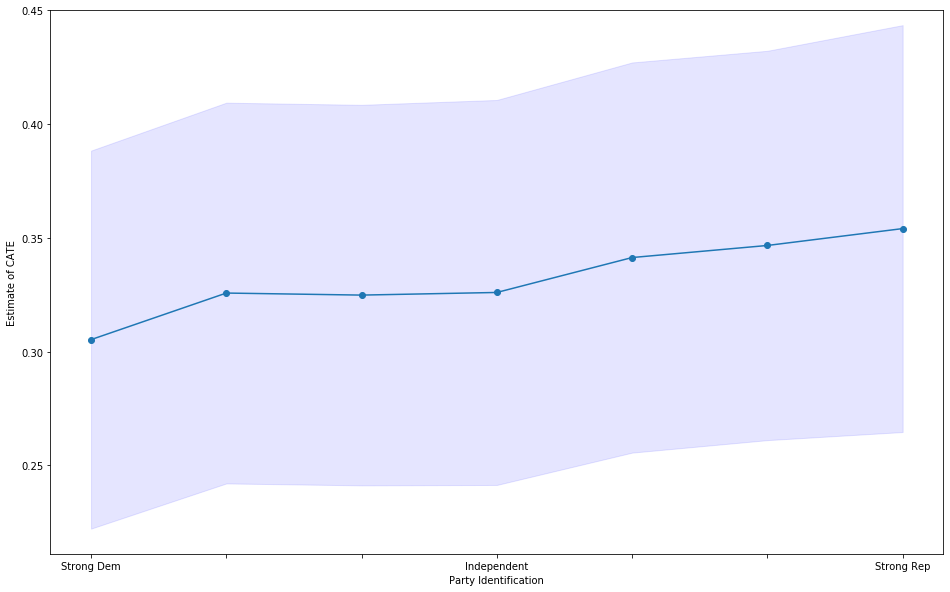
\includegraphics[width = \linewidth]{Graphs/s1_partyid.png}
		\vspace{0.5cm}
	\end{subfigure}
	\begin{subfigure} [h] {0.45\linewidth}
		\caption{\textbf{Political Views}}
   	 	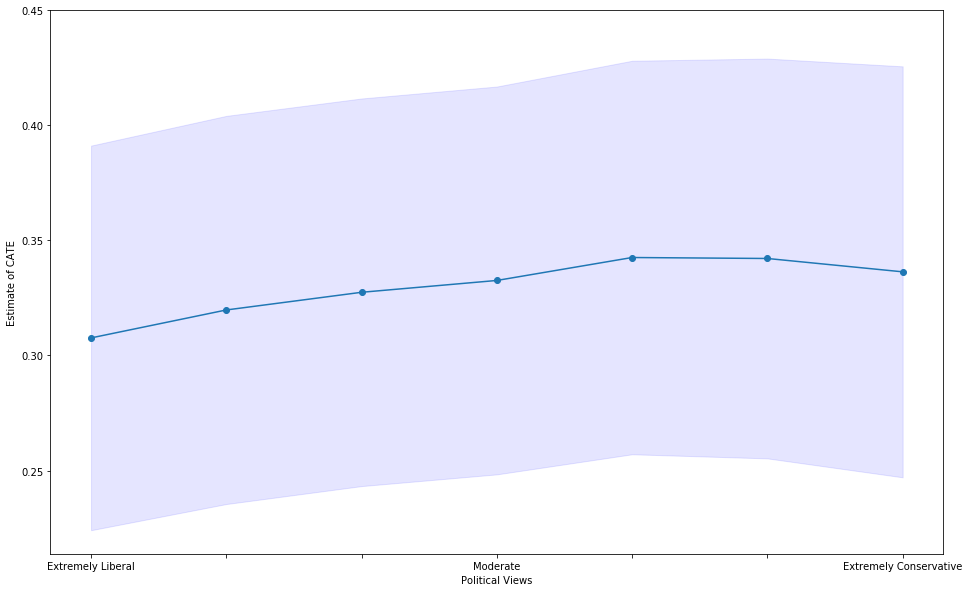
\includegraphics[width = \linewidth]{Graphs/s1_polyview.png}
		\vspace{0.5cm}
	\end{subfigure}}
\resizebox*{\textwidth}{!}{
	\begin{subfigure} [h] {0.45\linewidth}
	\caption{\textbf{Age }}
   	 	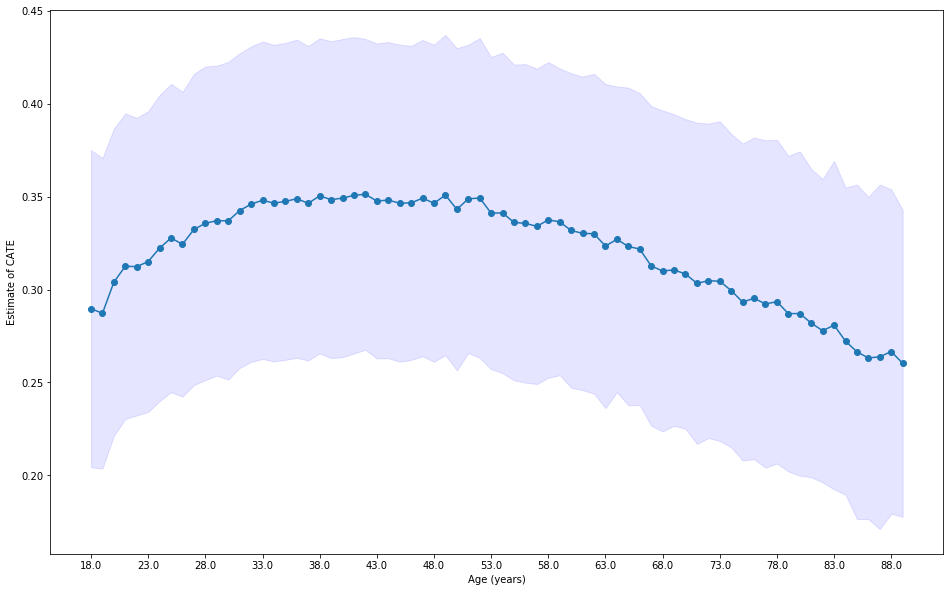
\includegraphics[width = \linewidth]{Graphs/s1_age.png}
		\vspace{0.5cm}
	\end{subfigure}
	\begin{subfigure} [h] {0.45\linewidth}
		\caption{\textbf{Education Received}}
   	 	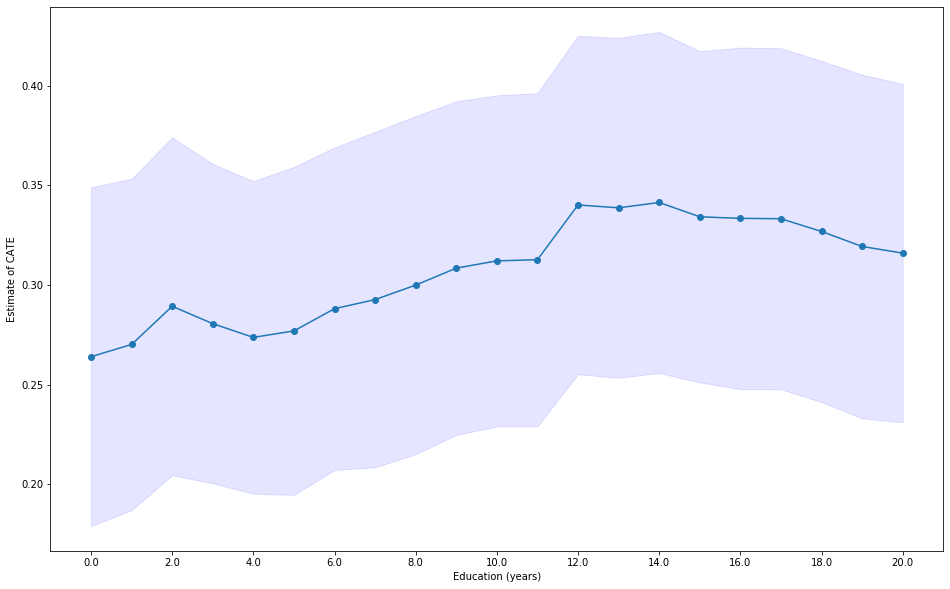
\includegraphics[width = \linewidth]{Graphs/s1_educ.png}
		\vspace{0.5cm}
	\end{subfigure}}
\resizebox*{\textwidth}{!}{
	\begin{subfigure} [h] {0.45\linewidth}
	\caption{\textbf{Attitude Toward Blacks}}
   	 	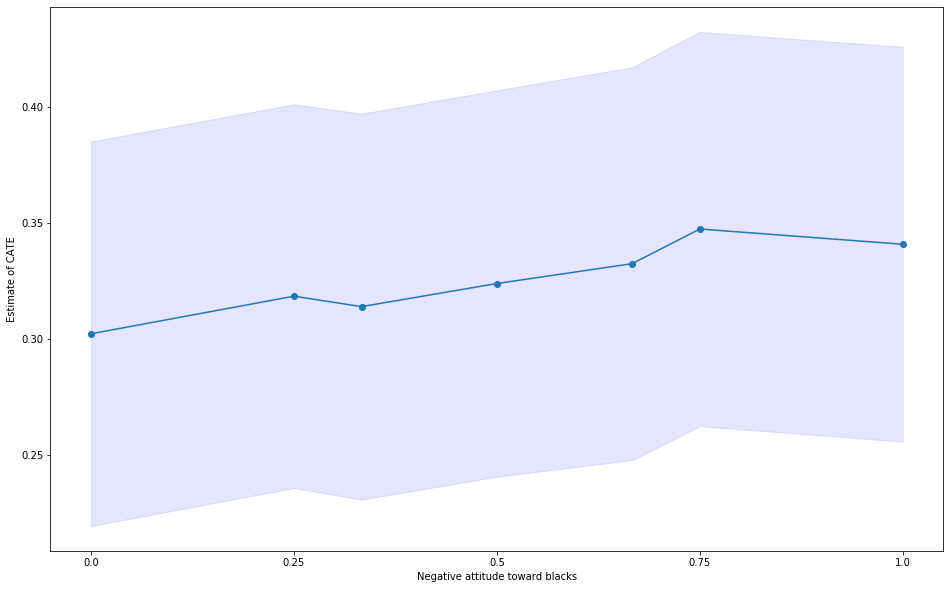
\includegraphics[width = \linewidth]{Graphs/s1_attblack.png}
		\vspace{0.5cm}
	\end{subfigure}
	\begin{subfigure} [h] {0.45\linewidth}
		\caption{\textbf{Survey Year}}
   	 	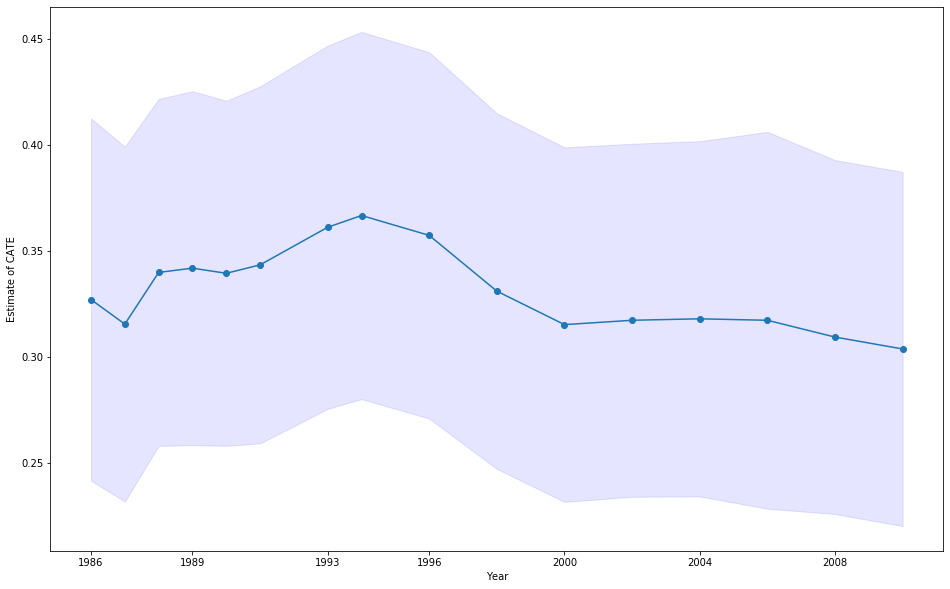
\includegraphics[width = \linewidth]{Graphs/s1_year.png}
		\vspace{0.5cm}
	\end{subfigure}}
\footnotesize
\emph{Notes:}  Each y-axis shows the estimated CATE conditioned on the covariate, each x-axis represents the range of covariate values for which the CATE was estimated.
\end{figure} 

\begin{figure}[!htp]
\caption{\label{figure:two}Histogram of CATE Estimates}
	\centering
   	 	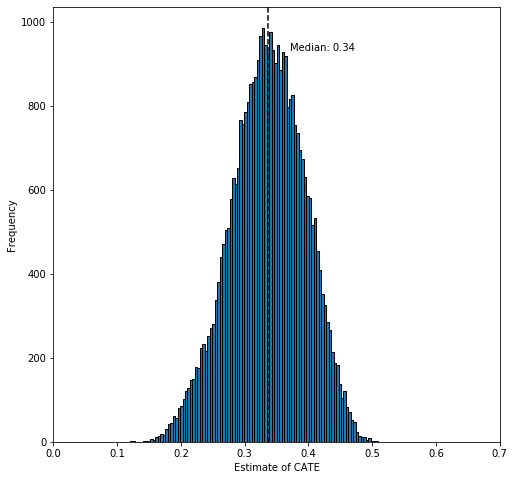
\includegraphics[width = 0.6\linewidth]{Graphs/s1_catefreq.png}
\end{figure} 

\begin{figure}[!htp]
\caption{\label{figure:three}Summary of SHAP Values of Covariate Importance}
	\centering
   	 	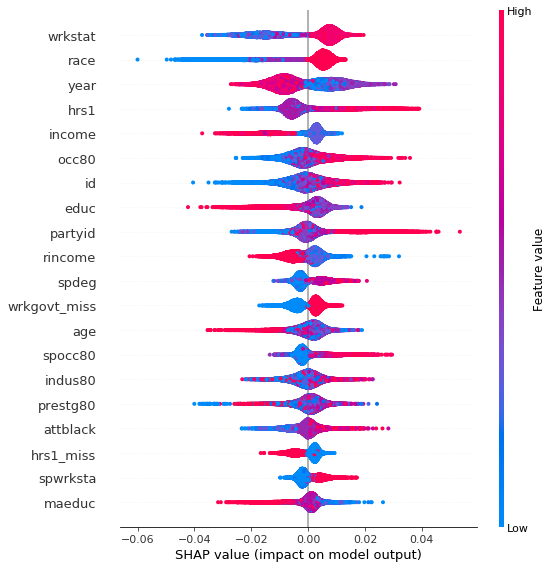
\includegraphics[width = 0.6\linewidth]{Graphs/s1_shap.png}
\end{figure} 

\begin{figure}[!htp]
\caption{\label{figure:four}Estimated vs. Actual CATE across Race Groups}
	\centering
	\begin{subfigure} [h] {0.49\linewidth}
		\caption{\textbf{1000 Samples}}
   	 	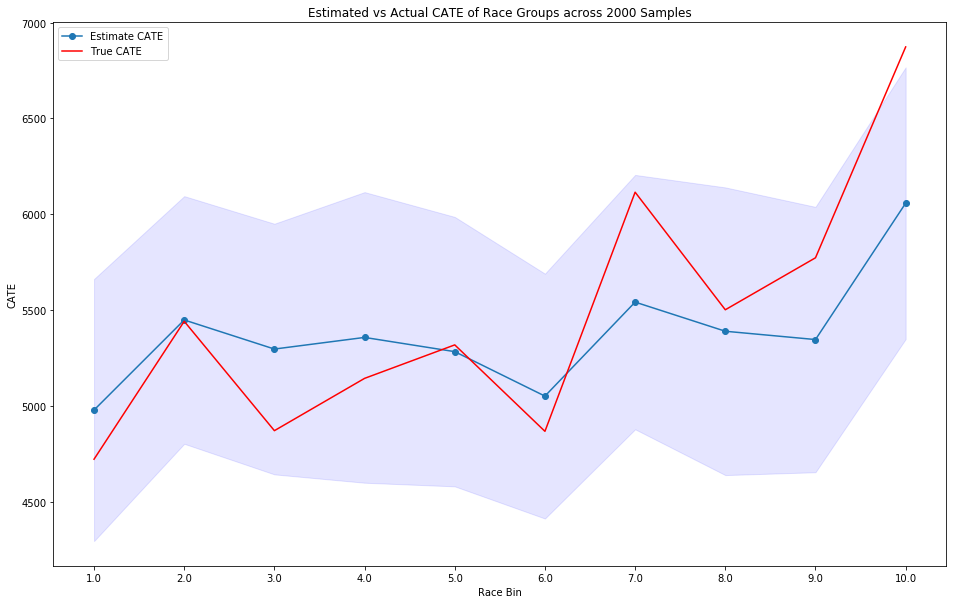
\includegraphics[width = \linewidth]{Graphs/s2_race2000.png}
	\end{subfigure}
	\begin{subfigure} [h] {0.49\linewidth}
		\caption{\textbf{30000 Samples}}
   	 	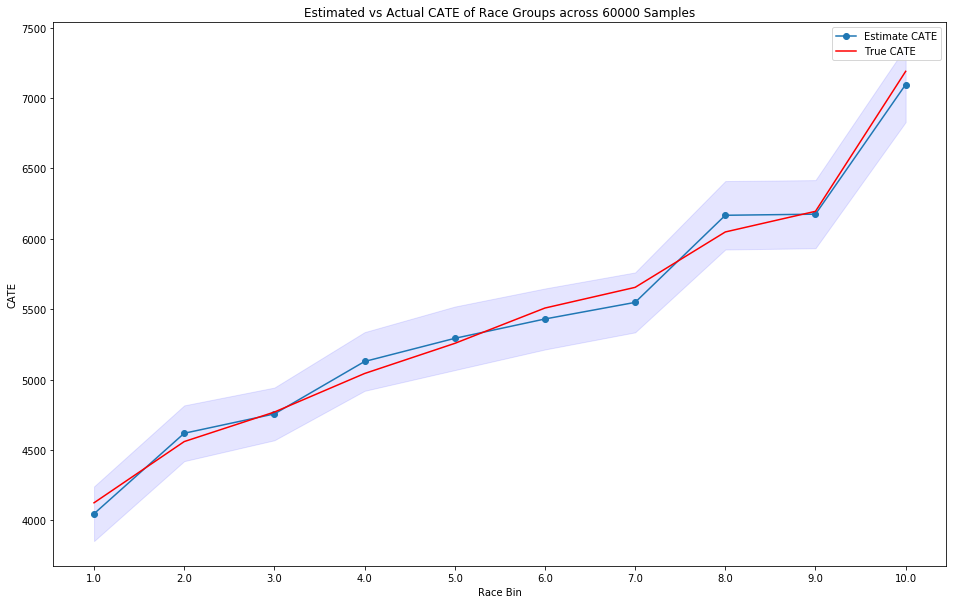
\includegraphics[width = \linewidth]{Graphs/s2_race60000.png}
	\end{subfigure}
\footnotesize
\emph{Notes:}  y-axis is the CATE, x-axis the range of covariate values split into bins on which CATE is estimated. The red line is the true CATE and blue line is the estimate CATE with the shaded area representing the 95\% CI.
\end{figure} 

\begin{figure}[!htp]
\caption{\label{figure:five}Estimated vs. Actual CATE across Education Level}
	\centering
	\begin{subfigure} [h] {0.49\linewidth}
		\caption{\textbf{1000 Samples}}
   	 	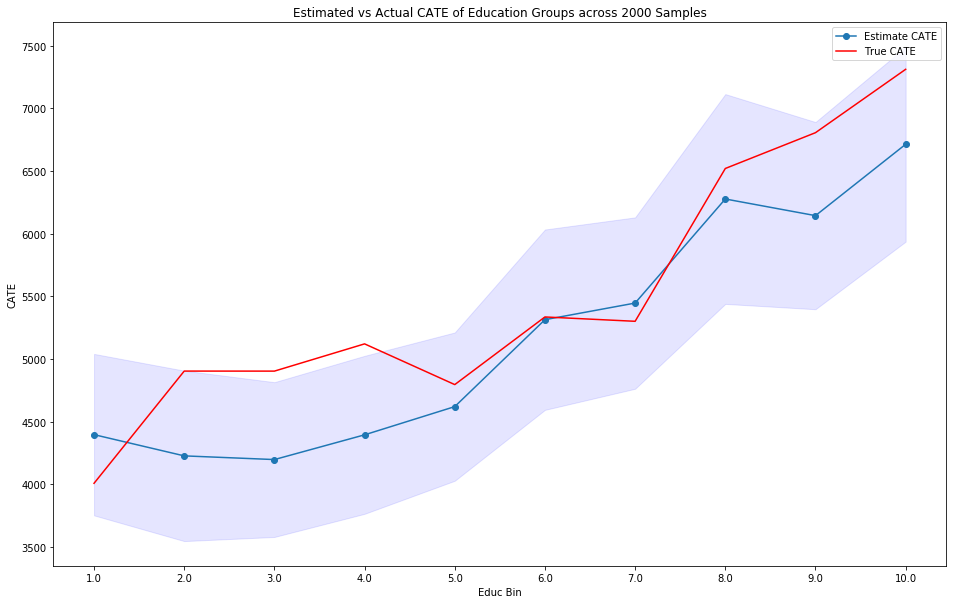
\includegraphics[width = \linewidth]{Graphs/s2_educ2000.png}
	\end{subfigure}
	\begin{subfigure} [h] {0.49\linewidth}
		\caption{\textbf{30000 Samples}}
   	 	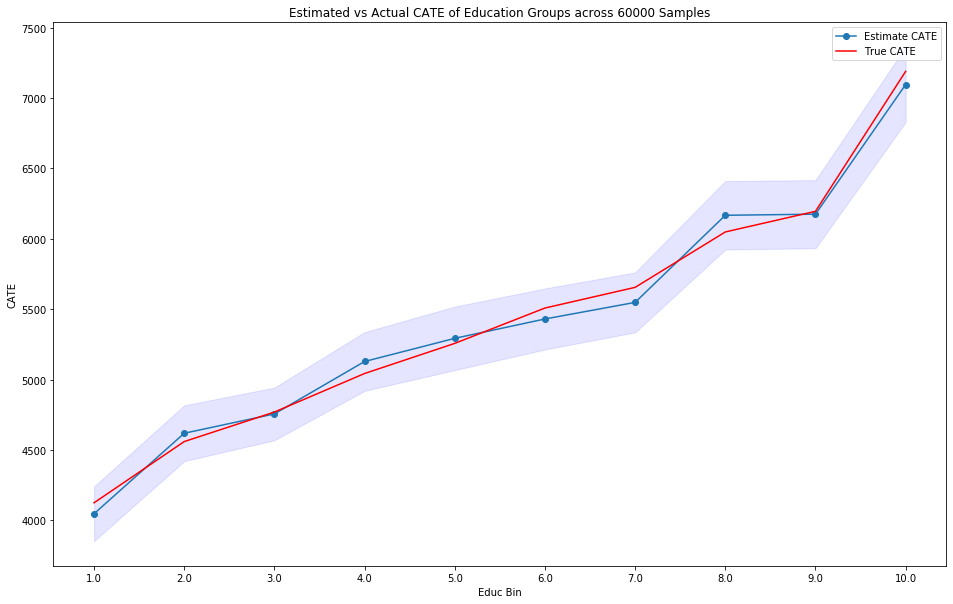
\includegraphics[width = \linewidth]{Graphs/s2_educ60000.png}
	\end{subfigure}
\footnotesize
\emph{Notes:}  y-axis is the CATE, x-axis the range of covariate values split into bins on which CATE is estimated. The red line is the true CATE and blue line is the estimate CATE with the shaded area representing the 95\% CI.
\end{figure} 

\begin{figure}[!htp]
\caption{Relative Model Performance by Parameter Variation }
	\centering
	\begin{subfigure} [h] {\linewidth}
		\caption{\label{figure:sixa}\textbf{Sample Size}}
   	 	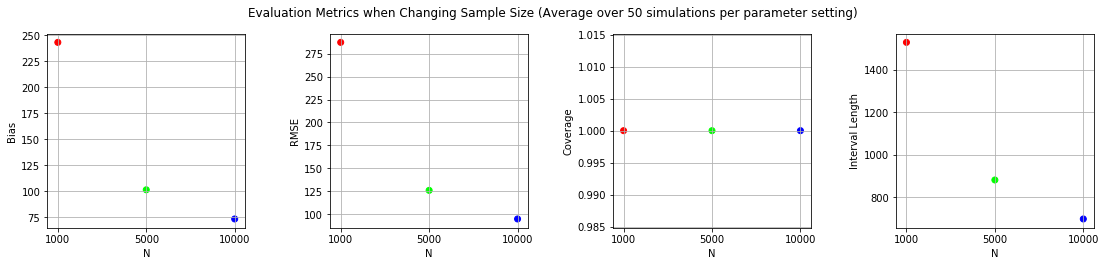
\includegraphics[width = \linewidth]{Graphs/s2_nsiz.png}
	\end{subfigure}
	\begin{subfigure} [h] {\linewidth}
\vspace{0.5cm}
		\caption{\label{figure:sixb}\textbf{Linearity}}
   	 	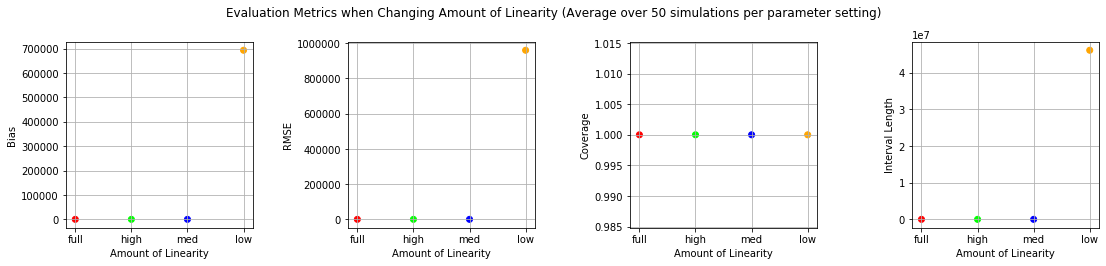
\includegraphics[width = \linewidth]{Graphs/s2_linear.png}
	\end{subfigure}
	\begin{subfigure} [h] {\linewidth}
\vspace{0.5cm}
		\caption{\label{figure:sixc}\textbf{Propensity Score}}
   	 	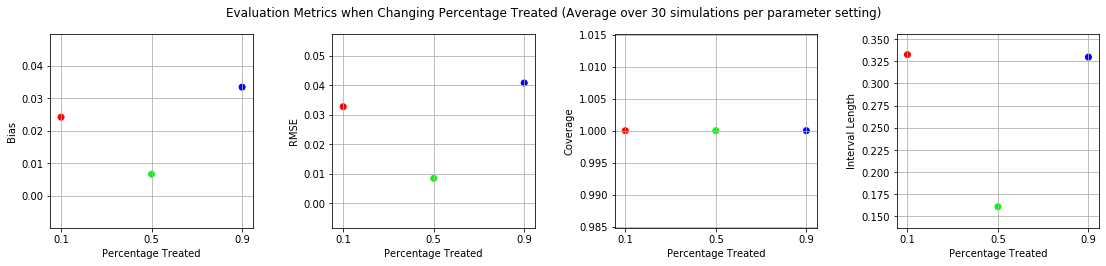
\includegraphics[width = \linewidth]{Graphs/s2_propen.png}
	\end{subfigure}
	\begin{subfigure} [h] {\linewidth}
\vspace{0.5cm}
		\caption{\label{figure:sixd}\textbf{Overlap}}
   	 	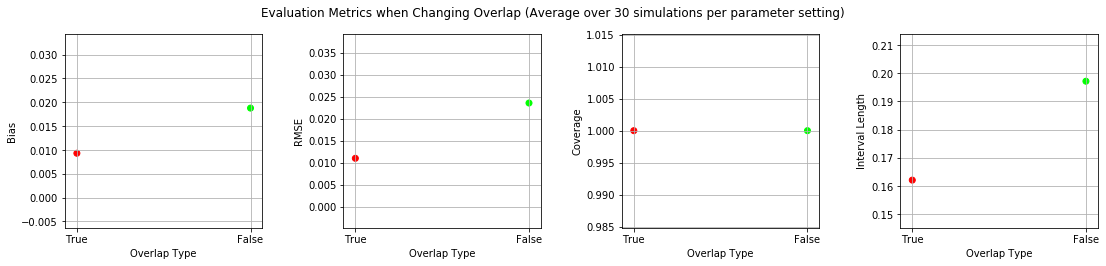
\includegraphics[width = \linewidth]{Graphs/s2_overlap.png}
	\end{subfigure}
\end{figure} 

\begin{figure}
\ContinuedFloat
	\begin{subfigure} [!ht] {\linewidth}
		\caption{\label{figure:sixe}\textbf{Degree of Heterogeneity}}
   	 	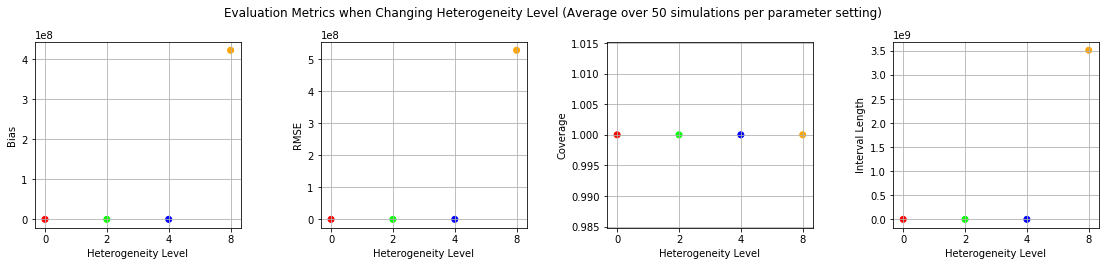
\includegraphics[width = \linewidth]{Graphs/s2_hetero.png}
	\end{subfigure}
	\begin{subfigure} [!ht] {\linewidth}
\vspace{0.5cm}
		\caption{\label{figure:sixf}\textbf{Number of Estimators}}
   	 	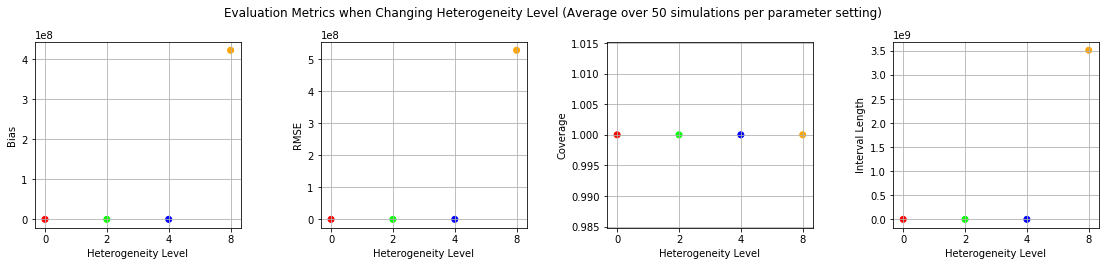
\includegraphics[width = \linewidth]{Graphs/s2_nestimator.png}
	\end{subfigure}
\end{figure} 

\begin{figure}[!htp]
\caption{\label{figure:seven}CATE Estimates by Variation in Degrees of Heterogeneity}
	\centering
	\begin{subfigure} [h] {0.49\linewidth}
		\caption{\textbf{\textit{j = 0} (Homogeneity)}}
   	 	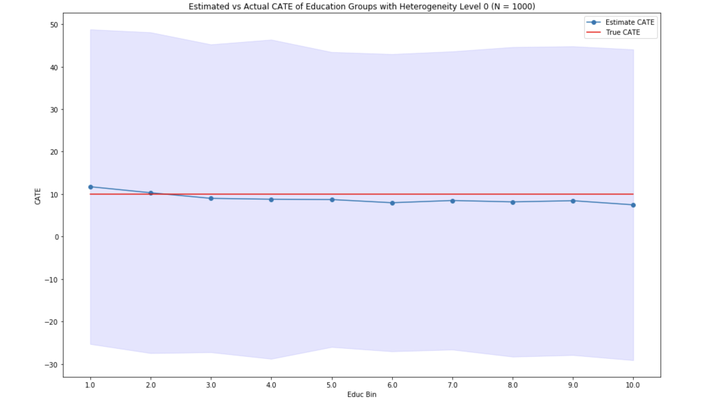
\includegraphics[width = \linewidth]{Graphs/s2_CATEhet0.png}
	\end{subfigure}
	\begin{subfigure} [h] {0.49\linewidth}
		\caption{\textit{j = 2}}
   	 	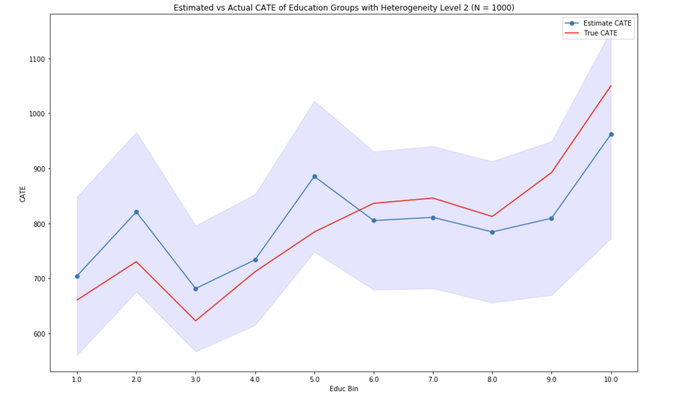
\includegraphics[width = \linewidth]{Graphs/s2_CATEhet2.png}
	\end{subfigure}
	\begin{subfigure} [h] {0.49\linewidth}
	\vspace{0.5cm}
		\caption{\textit{j = 4}}
   	 	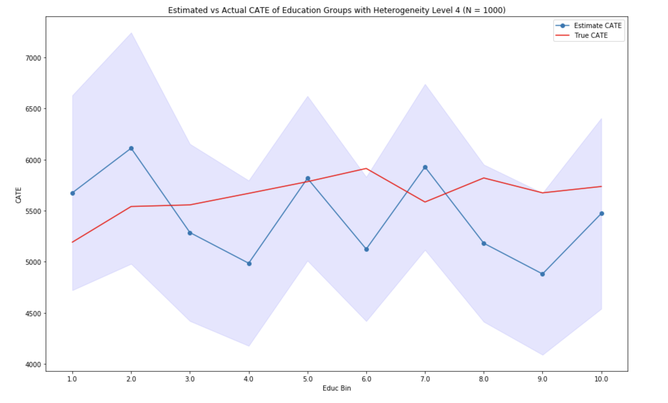
\includegraphics[width = \linewidth]{Graphs/s2_CATEhet4.png}
	\end{subfigure}
	\begin{subfigure} [h] {0.49\linewidth}
	\vspace{0.5cm}
		\caption{\textit{j = 8}}
   	 	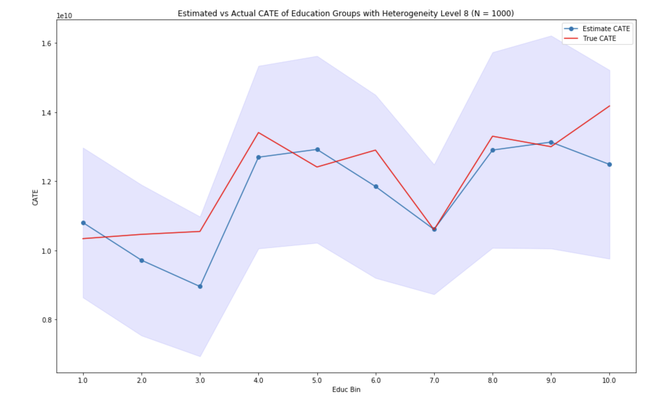
\includegraphics[width = \linewidth]{Graphs/s2_CATEhet8.png}
	\end{subfigure}
\end{figure} 



\clearpage
\bibliographystyle{abbrv}
\bibliography{Bibliography}


\clearpage
\appendix
\section{References from Green and Kern (2012) }

\begin{figure}[!ht]
\renewcommand{\thefigure}{A1}
\caption{\label{figure:GK}CATE Estimates Obtained by BART}
	\centering
   	 	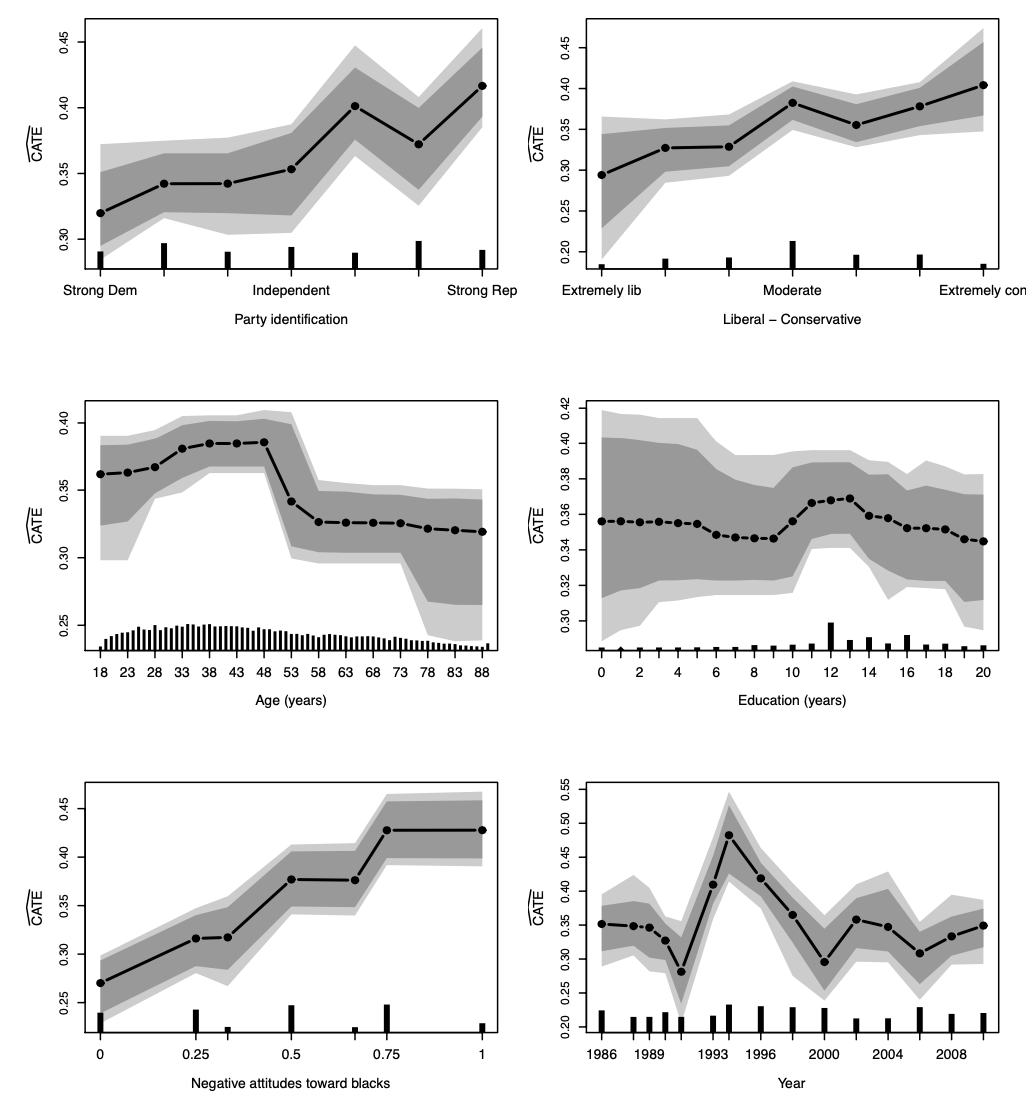
\includegraphics[width = 0.6\linewidth]{Graphs/A_GK_cate.png} \\
\footnotesize
\emph{Notes:} Source: Green and Kern (2012). GSS 1986–2010. CATE estimates (on the probability scale) are shown. The dark grey areas are point-wise 95\% posterior bands; the light grey areas are global 95\% posterior bands. Marginal covariate distributions are displayed at the bottom of the graphs.
\end{figure} 

\begin{figure}[!ht]
\renewcommand{\thefigure}{A2}
\caption{Histogram of CATE Estimates (BART)}
	\centering
   	 	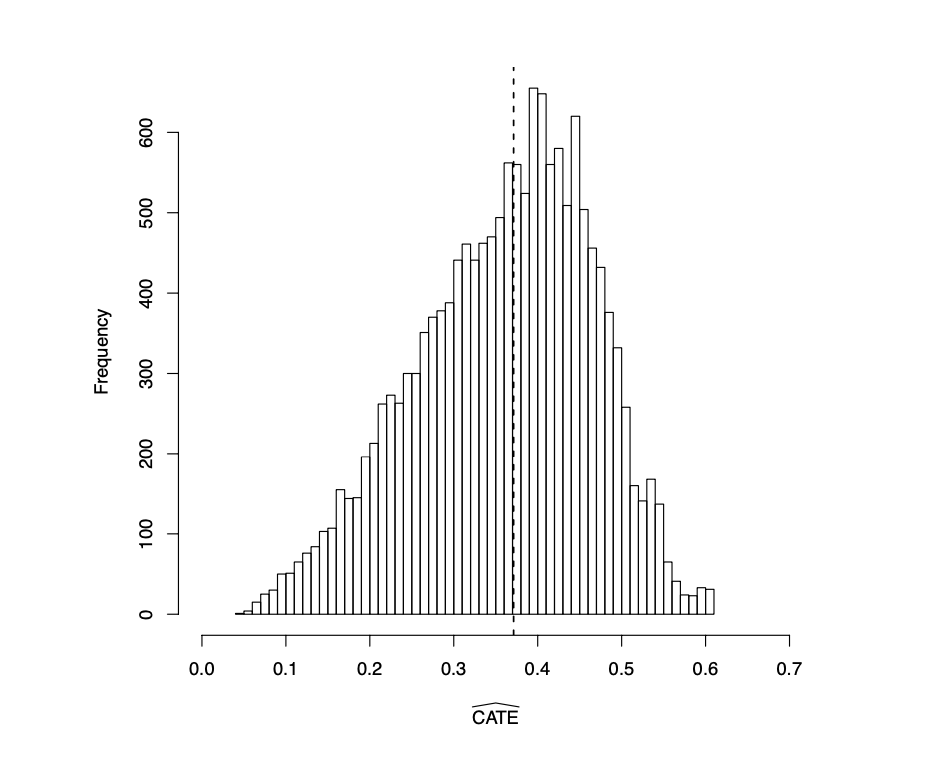
\includegraphics[width = 0.6\linewidth]{Graphs/A_GK_catefreq.png} \\ 
\footnotesize
\emph{Notes:} Source: Green and Kern (2012). GSS 1986–2010. The graph displays a histogram of CATE estimates (on the probability scale). The vertical dashed line denotes the median CATE estimate.
\end{figure} 


\end{document}



















